

%%%%%%%%%%%%%%%%%%%%%%%%%%%%%%%%%%% How-To: ViennaCL basics %%%%%%%%%%%%%%%%%%%%%%%%%%%%%%%%%%%%



\begin{frame}{ }
 \begin{center}
  \Large \textbf{How-To: \ViennaCL \ Basics}
 \end{center}
\end{frame}


\begin{frame}{How-To: \ViennaCL \ Basics}

\begin{block}{What to expect}
  \begin{itemize}
   \item From BLAS to Boost.uBLAS to ViennaCL
   \item Basic Types
   \item OpenCL Kernels
   \item Basic Usage: Data Management
   \item Basic Usage: Algebra
   \item Basic Usage: Solver
   \item Summary
  \end{itemize}
\end{block}

\end{frame}



\begin{frame}{From BLAS to Boost.uBLAS to ViennaCL}

\begin{block}{BLAS}
  \begin{itemize}
   \item \textbf{B}asic \textbf{L}inear \textbf{A}lgebra \textbf{S}ubprograms
   \item De facto API standard
   \item Low level interface
  \end{itemize}
\end{block}

\begin{block}{Boost.uBLAS}
  \begin{itemize}
   \item C++ API for BLAS
   \item High level interface
   \item Part of Boost libraries
  \end{itemize}
\end{block}

\end{frame}



\begin{frame}[fragile]
\frametitle{From BLAS to Boost.uBLAS to ViennaCL}
\begin{block}{Consider Existing CPU Code (Boost.uBLAS)}
  \begin{lstlisting}
using namespace boost::numeric::ublas;

matrix<double> A(1000, 1000);
vector<double> x(1000), rhs(1000);

/* Fill A, x, rhs here */

rhs += 2.0 * x;
double val = inner_prod(x, rhs);
matrix += val * outer_prod(x, rhs);

x = solve(A, rhs, upper_tag()); // Upper triangular solver

std::cout << "  2-norm: " << norm_2(x) << std::endl;
std::cout << "sup-norm: " << norm_inf(x) << std::endl;
  \end{lstlisting}
\end{block}

\begin{block}{High-Level Code with Syntactic Sugar}
\end{block}

\end{frame}


\begin{frame}{From BLAS to Boost.uBLAS to ViennaCL}

  \begin{block}{Porting the previous code to GPU}
  \end{block}

  \begin{block}{``How much time will you need{?}``}
    \begin{itemize}
     \item 1 minute?
     \item 1 hour?
     \item 1 day?
    \end{itemize}
  \end{block}

  \begin{block}{Quality Criteria}
   \begin{itemize}
     \item Working hours spent
     \item Performance
     \item Correctness
     \item High-level description (Maintainability)
   \end{itemize}
  \end{block}

\end{frame}


\begin{frame}[fragile]
\frametitle{From BLAS to Boost.uBLAS to ViennaCL}
\begin{block}{Consider Existing CPU Code (Boost.uBLAS)}
  \begin{lstlisting}
using namespace boost::numeric::ublas;


matrix<double> A(1000, 1000);
vector<double> x(1000), rhs(1000);

/* Fill A, x, rhs here */

rhs += 2.0 * x;
double val = inner_prod(x, rhs);
matrix += val * outer_prod(x, rhs);

x = solve(A, rhs, upper_tag()); // Upper triangular solver

std::cout << "  2-norm: " << norm_2(x) << std::endl;
std::cout << "sup-norm: " << norm_inf(x) << std::endl;
  \end{lstlisting}
\end{block}

\end{frame}

\begin{frame}[fragile]
\frametitle{From BLAS to Boost.uBLAS to ViennaCL}
 \begin{block}{Previous Code Snippet Rewritten with ViennaCL}
  \begin{lstlisting}
using namespace |\color{red}viennacl;|
using namespace |\color{red}viennacl::linalg;|

matrix<double> A(1000, 1000);
vector<double> x(1000), rhs(1000);

/* Fill A, x, rhs here */

rhs += 2.0 * x;
double val = inner_prod(x, rhs);
matrix += val * outer_prod(x, rhs);

x = solve(A, rhs, upper_tag()); // Upper triangular solver

std::cout << "  2-norm: " << norm_2(x) << std::endl;
std::cout << "sup-norm: " << norm_inf(x) << std::endl;
  \end{lstlisting} 
 \end{block}
\end{frame}



%%%%%%%%%%%%%%% Iterative solvers %%%%%%%%%%%%%%%%%%%%%%
\begin{frame}[fragile]
\frametitle{From BLAS to Boost.uBLAS to ViennaCL}
\begin{block}{ViennaCL in addition provides iterative solvers}
  \begin{lstlisting}
using namespace viennacl;
using namespace viennacl::linalg;

compressed_matrix<double> A(1000, 1000);
vector<double> x(1000), rhs(1000);

/* Fill A, x, rhs here */

x = solve(A, rhs, cg_tag()); // Conjugate Gradient solver
x = solve(A, rhs, bicgstab_tag()); // BiCGStab solver
x = solve(A, rhs, gmres_tag());    // GMRES solver
  \end{lstlisting}
\end{block}

 \begin{block}{No iterative solvers available in uBLAS...}
 \end{block}
\end{frame}


\begin{frame}[fragile]
\frametitle{From BLAS to Boost.uBLAS to ViennaCL}
\begin{block}{Thanks to interface compatibility}
  \begin{lstlisting}
using namespace |\color{red}boost::numeric::ublas;|
using namespace viennacl::linalg;

compressed_matrix<double> A(1000, 1000);
vector<double> x(1000), rhs(1000);

/* Fill A, x, rhs here */

x = solve(A, rhs, cg_tag()); // Conjugate Gradient solver
x = solve(A, rhs, bicgstab_tag()); // BiCGStab solver
x = solve(A, rhs, gmres_tag());    // GMRES solver
  \end{lstlisting} 
\end{block}

\vspace{1.15cm}

\end{frame}



\begin{frame}[fragile]
\frametitle{OpenCL kernels}

\begin{block}{OpenCL kernels are needed for actual computation}
  \begin{itemize}
   \item Provided by ViennaCL
   \item Support for expression templates
   \item Automatic kernel generation
  \end{itemize}
\end{block}

\begin{block}{Each of the following commands launches a separate OpenCL kernel}
\begin{lstlisting}
v1 = v2;
v1 += v2;
v1 -= v2;
v1 = alpha * v2;
v1 += alpha * v2;
v1 -= alpha * v2;
v1 *= alpha;
v1 /= alpha;
\end{lstlisting}
\end{block}

\end{frame}


\begin{frame}[fragile]
\frametitle{OpenCL kernels}

\begin{block}{OpenCL kernels have to be compiled at run time}
\begin{itemize}
  \item OpenCL JIT compiler
  \item Kernels can be grouped in programs
\end{itemize}
\end{block}

\begin{block}{Compilation strategies}
\begin{itemize}
  \item Each kernel individually: several milliseconds per kernel
  \item All at once: Takes seconds
  \item In groups: Compile groups of kernels whenever potentially needed
\end{itemize}
\end{block}

\end{frame}


\begin{frame}[fragile]
\frametitle{OpenCL kernels}

\begin{block}{Consider the following code}
  \begin{lstlisting}
int main(){
  vector<double> x(100), y(100);
  matrix<double> A(100, 100), B(100, 100);
  matrix<double, column_major> C(100, 100);

  x += 3.1415 * y;
  C = prod(trans(A), B);
  y = prod(C, x);

  std::cout << y << std::endl;
}
  \end{lstlisting}
\end{block}

\begin{block}{OpenCL Kernels}
  \begin{itemize}
    \item Which kernels are compiled?
    \item When are they compiled?
    \item Hint: Program compiles and executes normally
  \end{itemize}
\end{block}

\end{frame}


\begin{frame}[fragile]
\frametitle{OpenCL kernels}

\begin{block}{Consider the following code}
  \begin{lstlisting}
int main(){
  |\color{red}vector<double> x(100), y(100);|
  |\color{red}matrix<double> A(100, 100), B(100, 100);|
  |\color{red}matrix<double, column\_major> C(100, 100);|

  x += 3.1415 * y;
  C = prod(trans(A), B);
  y = prod(C, x);

  std::cout << y << std::endl;
}
  \end{lstlisting}
\end{block}

\begin{block}{OpenCL Kernels}
  \begin{itemize}
    \item Which kernels are compiled?
    \item When are they compiled?
    \item Hint: Program compiles and executes normally
  \end{itemize}
\end{block}

\end{frame}



\begin{frame}[fragile]
\frametitle{OpenCL kernels}

\begin{block}{Consider the following code}
  \begin{lstlisting}
int main(){
  vector<double> x(100), y(100);
  matrix<double> A(100, 100), B(100, 100);
  matrix<double, column_major> C(100, 100);

  |\color{red}x += 3.1415 * y;|
  |\color{red}C = prod(trans(A), B);|
  |\color{red}y = prod(C, x);|

  std::cout << y << std::endl;
}
  \end{lstlisting}
\end{block}

\begin{block}{OpenCL Kernels}
  \begin{itemize}
    \item Which kernels are compiled?
    \item When are they compiled?
    \item Hint: Program compiles and executes normally
  \end{itemize}
\end{block}

\end{frame}


\begin{frame}{OpenCL kernel management}

\begin{block}{Special case: Matrix-Matrix product}
  \begin{itemize}
    \item Result matrix: Row/Column major memory layout
    \item First factor: Row/Column major, possibly transposed
    \item Second factor: Row/Column major, possibly transposed
  \end{itemize}
\end{block}

\begin{block}{Leads to 32 different kernels for matrix-matrix multiplication}
  \begin{itemize}
    \item Compiled separately on request
  \end{itemize}
\end{block}

\end{frame}



\begin{frame}{Basic Types}

\begin{block}{Supported types}
  \begin{itemize}
   \item Scalar
   \item Vector
   \item Dense matrix
   \item Sparse matrix
   \item Structured matrix
  \end{itemize}
\end{block}

\begin{block}{Numeric Types}
  \begin{itemize}
   \item float
   \item double
  \end{itemize}
\end{block}

\end{frame}



% \begin{frame}{Basic Types}
% 
% \TODO{Bild overview over types (scalar, vectors, matrices, dense matrices, sparse matrices, special types, ...)}
% 
% \end{frame}



\begin{frame}[fragile]
\frametitle{Basic Types}

\begin{block}{Scalars}  
  \begin{itemize}
   \item Represents a single scalar value on the computing device
   \item Behave like underlying type
   \item Implicit cast to underlying type
   \item Potentially expensive (Overhead!)
  \end{itemize}
  
  \begin{lstlisting}
viennacl::scalar<NumericType> gpu_scalar;
viennacl::scalar<float> gpu_float;
viennacl::scalar<double> gpu_double;
  \end{lstlisting}
\end{block}

\end{frame}



\begin{frame}[fragile]
\frametitle{Basic Types}
\begin{block}{Scalars}
  \begin{lstlisting}
float cpu_float = 42.0f;
double cpu_double = 13.7603;
viennacl::scalar<float> gpu_float(3.1415f);
viennacl::scalar<double> gpu_double = 2.71828;

// conversions and t
cpu_float = gpu_float;
// automatic transfer and conversion
gpu_float = cpu_double;

cpu_float = gpu_float * 2.0f;
cpu_double = gpu_float - cpu_float;
  \end{lstlisting}
\end{block}
\end{frame}



\begin{frame}[fragile]
\frametitle{Basic Types}

\begin{block}{Vectors}  
  \begin{itemize}
   \item Represents a vector on the computing device
   \item Operator overloading
   \item Alignment support
  \end{itemize}
  
  \begin{lstlisting}
viennacl::vector<NumericType> gpu_vector;

viennacl::vector<float> gpu_float_vector;
viennacl::vector<double> gpu_double_vector;
  \end{lstlisting}
\end{block}

\end{frame}



\begin{frame}[fragile]
\frametitle{Basic Types}

\begin{block}{Vectors}
  \begin{lstlisting}
std::vector<ScalarType> stl_vec(10);
viennacl::vector<ScalarType> vcl_vec(10);

//fill the STL vector:
for (unsigned int i=0; i<vector_size; ++i)
  stl_vec[i] = i;

//copy content to GPU vector (recommended initialization)
copy(stl_vec.begin(), stl_vec.end(), vcl_vec.begin());

//manipulate GPU vector here
vcl_vec *= 4.2;

//copy content from GPU vector back to STL vector
copy(vcl_vec.begin(), vcl_vec.end(), stl_vec.begin());
  \end{lstlisting}
\end{block}

\end{frame}



\begin{frame}[fragile]
\frametitle{Basic Types}

\begin{block}{Vectors}
  \begin{lstlisting}
std::vector<ScalarType> stl_vec(10);
viennacl::vector<ScalarType> vcl_vec(10);

//fill the STL vector:
for (unsigned int i=0; i<vector_size; ++i)
  stl_vec[i] = i;

//copy content to GPU vector (recommended initialization)
copy(stl_vec, vcl_vec);

//manipulate GPU vector here
vcl_vec *= 4.2;

//copy content from GPU vector back to STL vector
copy(vcl_vec, stl_vec);
  \end{lstlisting}
\end{block}

\end{frame}




\begin{frame}[fragile]
\frametitle{Basic Types}

\begin{block}{Alignment}  
  \begin{itemize}
   \item Default = 1
   \item Template parameter
   \item In ViennaCL 1.5.0 deprecated (will be runtime parameter)
  \end{itemize}
  
  \begin{lstlisting}
viennacl::vector<NumericType, Alignment> gpu_vector_with_alignment;

viennacl::vector<float, 4>
    gpu_float_vector_with_alignment;

viennacl::vector<double, 8>
    gpu_double_vector_with_alignment;
  \end{lstlisting}
\end{block}

\end{frame}



\begin{frame}[fragile]
\frametitle{Basic Types}

\begin{block}{Vector initializer}  
  \begin{itemize}
   \item unit\_vector $\Rightarrow \textbf{u}_{N,i} = \left\{ \begin{array}{ll} 1 & \mbox{if $i = N$}; \\
                                                                     0 &  \mbox{else} \end{array} \right.$
   \item zero\_vector $\Rightarrow \textbf{z}_i = 0$
   \item scalar\_vector $\Rightarrow \textbf{s}_i = s$
  \end{itemize}
  
  \begin{lstlisting}
viennacl::unit_vector<NumericType>(size, index);
    
viennacl::zero_vector<NumericType>(size);
    
viennacl::scalar_vector<NumericType>(size, scalar);
  \end{lstlisting}
\end{block}

\end{frame}



\begin{frame}[fragile]
\frametitle{Basic Types}

\begin{block}{Vector initializer}
  \begin{lstlisting}
viennacl::vector<ScalarType> vcl_vec =
    viennacl::unit_vector<ScalarType>(10, 5);
// Creates the vector (0, 0, 0, 0, 1, 0, 0, 0, 0, 0)

viennacl::vector<ScalarType> vcl_vec =
    viennacl::zero_vector<ScalarType>(10);
// Creates the vector (0, 0, 0, 0, 0, 0, 0, 0, 0, 0)

viennacl::vector<ScalarType> vcl_vec =
    viennacl::scalar_vector<ScalarType>(6, 1.5);
// Creates the vector (1.5, 1.5, 1.5, 1.5, 1.5, 1.5)
  \end{lstlisting}
\end{block}

\end{frame}



\begin{frame}[fragile]
\frametitle{Basic Types}

\begin{block}{Dense matrix}  
  \begin{itemize}
   \item Represents a dense matrix on the computing device
   \item Dense matrix $\Rightarrow$ zero elements are rare
   \item Alignment support (same as vectors)
   \item Row major or column major
  \end{itemize}
  
  \begin{lstlisting}
viennacl::matrix<NumericType> gpu_matrix;
viennacl::matrix<NumericType, Scheme, Alignment>
    gpu_matrix_with_scheme_and_alignment;

viennacl::matrix<float> gpu_float_matrix;
viennacl::matrix<float, row_major, 4>
    row_major_gpu_float_matrix_with_alignment;

viennacl::matrix<double> gpu_double_matrix;
viennacl::matrix<double, column_major, 8>
    column_major_gpu_double_matrix_with_alignment;
  \end{lstlisting}
\end{block}

\end{frame}




\begin{frame}[fragile]
\frametitle{Basic Types}

\begin{block}{Dense matrix}
  \begin{lstlisting}
//set up a 3 by 5 matrix:
viennacl::matrix<float> vcl_matrix(4, 5);
//fill it up:
vcl_matrix(0,2) =  1.0
vcl_matrix(1,2) = -1.5;
vcl_matrix(2,0) =  4.2;
vcl_matrix(3,4) =  3.1415;
  \end{lstlisting}
\end{block}

\end{frame}



\begin{frame}[fragile]
\frametitle{Basic Types}

\begin{block}{Matrix initializer}  
  \begin{itemize}
   \item identity\_matrix $\Rightarrow \textbf{I}_{i,j} = \left\{ \begin{array}{ll} d & \mbox{if $i = j$}; \\
                                                                     0 &  \mbox{else} \end{array} \right.$
   \item zero\_matrix $\Rightarrow \textbf{Z}_{i,j} = 0$
   \item scalar\_matrix $\Rightarrow \textbf{S}_{i,j} = s$
  \end{itemize}
  
  \begin{lstlisting}
viennacl::identity_matrix<NumericType>(size, diagonal);
    
viennacl::zero_matrix<NumericType>(row_number, column_number);
    
viennacl::scalar_matrix<NumericType>(row_number, column_number, scalar);
  \end{lstlisting}
\end{block}

\end{frame}



\begin{frame}[fragile]
\frametitle{Basic Types}

\begin{block}{Matrix initializer}
  \begin{lstlisting}
viennacl::matrix<ScalarType> vcl_mat =
    viennacl::identity_matrix<ScalarType>(4, 1);
  \end{lstlisting}
  
  \hspace{1cm}
  
  Creates the following matrix:
$\begin{pmatrix}
1 & 0 & 0 & 0 \\
0 & 1 & 0 & 0 \\
0 & 0 & 1 & 0 \\
0 & 0 & 0 & 1
\end{pmatrix}$
\end{block}

\end{frame}



\begin{frame}[fragile]
\frametitle{Basic Types}

\begin{block}{Matrix initializer}
  \begin{lstlisting}
viennacl::matrix<ScalarType> vcl_mat =
    viennacl::zero_matrix<ScalarType>(3, 5);
  \end{lstlisting}
  
  \hspace{1cm}
  
  Creates the following matrix:
$\begin{pmatrix}
0 & 0 & 0 & 0 & 0 & 0 \\
0 & 0 & 0 & 0 & 0 & 0 \\
0 & 0 & 0 & 0 & 0 & 0
\end{pmatrix}$
\end{block}

\end{frame}



\begin{frame}[fragile]
\frametitle{Basic Types}

\begin{block}{Matrix initializer}
  \begin{lstlisting}
viennacl::matrix<ScalarType> vcl_mat =
    viennacl::scalar_matrix<ScalarType>(4, 3, 4.2);
  \end{lstlisting}
  
  \hspace{1cm}
  
  Creates the following matrix:
$\begin{pmatrix}
4.2 & 4.2 & 4.2 \\
4.2 & 4.2 & 4.2 \\
4.2 & 4.2 & 4.2 \\
4.2 & 4.2 & 4.2
\end{pmatrix}$
\end{block}

\end{frame}



\begin{frame}
\frametitle{Basic Types}

\begin{block}{Sparse matrix}
  \begin{itemize}
   \item Represents a sparse matrix on the computing device
   \item Sparse matrix $\Rightarrow$ zero elements are frequent
   \item Alignment support (same as vectors and dense matrices)
  \end{itemize}
\end{block}


\begin{block}{Sparse matrix types}
  \begin{itemize}
   \item Coordinate matrix
   \item Compressed matrix
   \item ELL matrix
   \item Hybrid matrix
  \end{itemize}
\end{block}

\end{frame}



\begin{frame}
\frametitle{Basic Types}

\begin{block}{Coordinate matrix}
  \begin{itemize}
   \item Easy to setup/extend
  \end{itemize}
  
  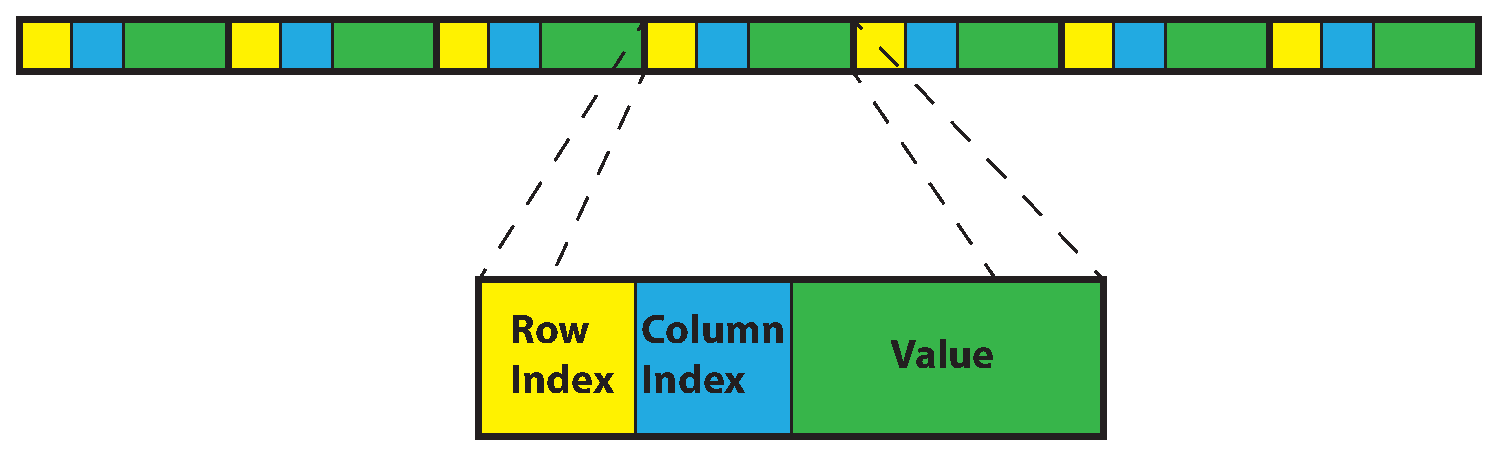
\includegraphics[width=0.8\textwidth]{figs/coordinate_matrix.eps}
\end{block}

\end{frame}



\begin{frame}
\frametitle{Basic Types}

\begin{block}{Compressed matrix}
  \begin{itemize}
    \item Less memory required
    \item Fast matrix-vector multiplication
  \end{itemize}
  
  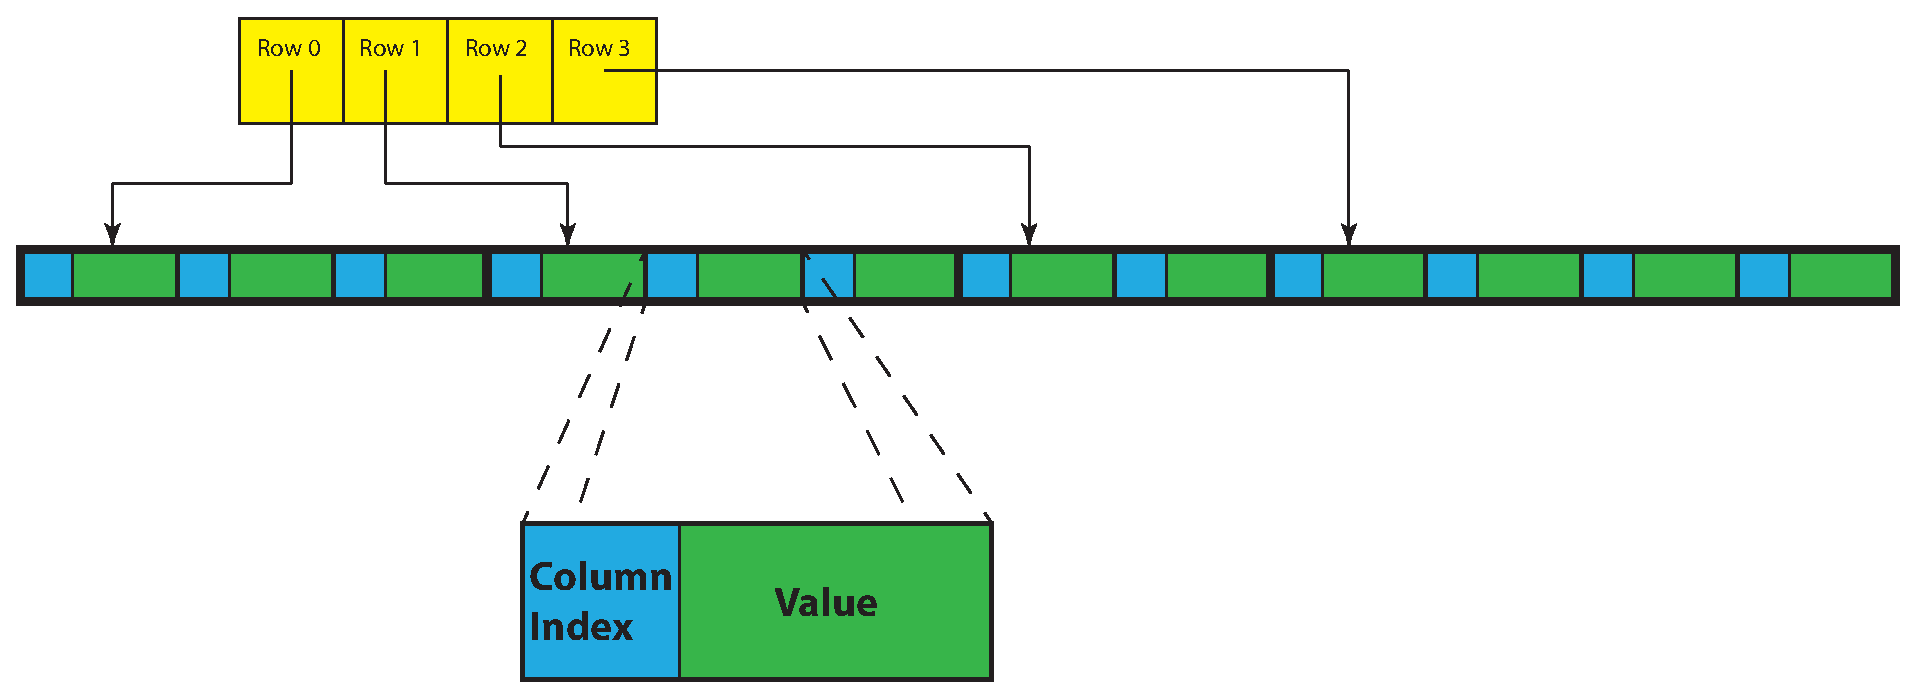
\includegraphics[width=0.8\textwidth]{figs/compressed_matrix.eps}
\end{block}

\end{frame}


\begin{frame}
\frametitle{Basic Types}

\begin{block}{ELL matrix}
  \begin{itemize}
    \item Similar to compressed matrix
    \item Fixed number of non-zero values per row
    \item No row jumper array required
  \end{itemize}
\end{block}

\begin{block}{Hybrid matrix}
  \begin{itemize}
    \item Combination of compressed matrix and ELL matrix
  \end{itemize}
\end{block}

\end{frame}



\begin{frame}[fragile]
\frametitle{Basic Types}

\begin{block}{Compressed matrix}
  \begin{lstlisting}
//set up a sparse 4 by 5 matrix on the CPU:
std::vector< std::map< unsigned int, float> >
    cpu_sparse_matrix(4);

//fill it up:
cpu_sparse_matrix[0][2] = 1.0;
cpu_sparse_matrix[1][2] = -1.5;
cpu_sparse_matrix[3][0] = 4.2;

//set up a sparse ViennaCL matrix:
viennacl::compressed_matrix<float> sparse_matrix(4, 5);

//copy to OpenCL device:
copy(cpu_sparse_matrix, sparse_matrix);

//copy back to CPU:
copy(sparse_matrix, cpu_sparse_matrix);
  \end{lstlisting}
\end{block}

\end{frame}





\begin{frame}
\frametitle{Basic Types}

\begin{block}{Structured matrix}
  \begin{itemize}
   \item Dense matrices but with special structure
   \item Access to one element might change other elements
  \end{itemize}
\end{block}

\begin{block}{Supported types}
  \begin{itemize}
   \item Circulant matrix
   \item Hankel matrix
   \item Toeplitz matrix
   \item Vandermonde matrix
  \end{itemize}
\end{block}

\end{frame}


\begin{frame}
\frametitle{Basic Types}

\begin{block}{Structured matrix}
  \begin{itemize}
   \item \textbf{Circulant matrix}
   \item Hankel matrix
   \item Toeplitz matrix
   \item Vandermonde matrix
  \end{itemize}
\end{block}

\begin{align*}
 \left( \begin{array}{ccccc}
         c_0 & c_{n-1} & \ldots & c_2 & c_1 \\
         c_1 & c_0 & c_{n-1} & & c_2 \\
         \vdots & c_1 & c_0 & \ddots & \vdots \\
         c_{n-2} & & \ddots & \ddots & c_{n-1} \\
         c_{n-1} & c_{n-2} & \hdots & c_1 & c_0 \\
        \end{array} \right)
\end{align*}

\end{frame}



\begin{frame}
\frametitle{Basic Types}

\begin{block}{Structured matrix}
  \begin{itemize}
   \item Circulant matrix
   \item \textbf{Hankel matrix}
   \item Toeplitz matrix
   \item Vandermonde matrix
  \end{itemize}
\end{block}

\begin{align*}
 \left( \begin{array}{cccc}
         a & b & c & d \\
         b & c & d & e \\
         c & d & e & f \\
         d & e & f & g \\
        \end{array} \right)
\end{align*}

\vspace{0.9cm}

\end{frame}


\begin{frame}
\frametitle{Basic Types}

\begin{block}{Structured matrix}
  \begin{itemize}
   \item Circulant matrix
   \item Hankel matrix
   \item \textbf{Toeplitz matrix}
   \item Vandermonde matrix
  \end{itemize}
\end{block}

\begin{align*}
 \left( \begin{array}{cccc}
         a & b & c & d \\
         e & a & b & c \\
         f & e & a & b \\
         g & f & e & a \\
        \end{array} \right)
\end{align*}

\vspace{0.9cm}

\end{frame}



\begin{frame}
\frametitle{Basic Types}

\begin{block}{Structured matrix}
  \begin{itemize}
   \item Circulant matrix
   \item Hankel matrix
   \item Toeplitz matrix
   \item \textbf{Vandermonde matrix}
  \end{itemize}
\end{block}

\begin{align*}
 \left( \begin{array}{ccccc}
         1 & \alpha_1 & \alpha_1^2 & \ldots & \alpha_1^{n-1} \\
         1 & \alpha_2 & \alpha_2^2 & \ldots & \alpha_2^{n-1} \\
         1 & \vdots & \vdots & \vdots \\
         1 & \alpha_m & \alpha_m^2 & \ldots & \alpha_m^{n-1} \\
        \end{array} \right)
\end{align*}

\vspace{0.6cm}

\end{frame}













\begin{frame}[fragile]
\frametitle{Basic Usage: Data Management}

\begin{block}{How to access/transfer ViennaCL vectors/matrices elements?}
  \begin{itemize}
   \item Direct element access
   \item
   \item
  \end{itemize}
  
  \begin{lstlisting}
vector<ScalarType> vcl(10);

for (int i = 0; i < 10; ++i)
    vcl(i) = i;
    
for (int i = 0; i < 10; ++i)
    std::cout << vcl(i) << std::endl;
  \end{lstlisting}
\end{block}

\vspace{1.15cm}

\end{frame}



\begin{frame}[fragile]
\frametitle{Basic Usage: Data Management}

\begin{block}{How to access/transfer ViennaCL vectors/matrices elements?}
  \begin{itemize}
   \item Direct element access
   \item Iterator
   \item
  \end{itemize}
  
  \begin{lstlisting}
vector<ScalarType> vcl(10);

ScalarType tmp = 0;
for (vector<ScalarType>::iterator it = vcl.begin();
    it != vcl.end(); ++it, tmp += 42.0)
    *it = tmp;
    
for (vector<ScalarType>::iterator it = vcl.begin();
    it != vcl.end(); ++it)
    std::cout << *it < std::endl;
  \end{lstlisting}
\end{block}

\end{frame}



\begin{frame}[fragile]
\frametitle{Basic Usage: Data Management}

\begin{block}{How to access/transfer ViennaCL vectors/matrices elements?}
  \begin{itemize}
   \item Direct element access
   \item Iterator
   \item Copy functions
  \end{itemize}
  
  \begin{lstlisting}
std::vector<ScalarType> cpu(10);
viennacl::vector<ScalarType> vcl(10);

for (int i = 0; i < 10; ++i)
    cpu[i] = i;
    
viennacl::copy( cpu.begin(), cpu.end(), vcl.begin() );

viennacl::copy( vcl.begin(), vcl.end(), cpu.begin() );
  \end{lstlisting}
\end{block}

\vspace{0.4cm}

\end{frame}



\begin{frame}[fragile]
\frametitle{Basic Usage: Data Management}

\begin{block}{How to access/transfer ViennaCL vectors/matrices elements?}
  \begin{itemize}
   \item Direct element access
   \item Iterator
   \item Copy functions
  \end{itemize}
  
  \begin{lstlisting}
std::vector<ScalarType> cpu(10);
viennacl::vector<ScalarType> vcl(10);

for (int i = 0; i < 10; ++i)
    cpu[i] = i;
    
viennacl::copy( cpu, vcl );

viennacl::copy( vcl, cpu );
  \end{lstlisting}
\end{block}

\vspace{0.4cm}

\end{frame}




\begin{frame}[fragile]
\frametitle{Basic Usage: Data Management}
 \begin{block}{Granularity of Operations}
  \begin{itemize}
   \item Filling a vector with data
   \begin{lstlisting}
viennacl::vector<double> v(10000);

for (size_t i=0; i<v.size(); ++i)
  v(i) = i;    
   \end{lstlisting}
  \end{itemize}
 \end{block}

%  \begin{block}{GPU Computing Is Fast, Right?}
%   \begin{center}
%   
\includegraphics[width=0.4\textwidth]{figs/fast.jpg}
%   \end{center}
%  \end{block}

\end{frame}


\begin{frame}[fragile]
\frametitle{Basic Usage: Data Management}
 \begin{block}{Granularity of Operations}
  \begin{itemize}
   \item Filling a vector with data
   \begin{lstlisting}
viennacl::vector<double> v(10000);

for (size_t i=0; i<v.size(); ++i)
  v(i) = i;    
   \end{lstlisting}
  \end{itemize}
 \end{block}

 \begin{block}{GPU Computing Is Fast, Right?}
  \begin{itemize}
   \item Execution time: 1 sec (approx)
   \item \texttt{std::vector}: $<$ 1 ms
  \end{itemize}

 \end{block}

 \vspace*{2.5cm}

\end{frame}

% \begin{frame}[fragile]
% \frametitle{Basic Usage: Data Management}
%  \begin{block}{Granularity of Operations}
%   \begin{itemize}
%    \item Filling a vector with data
%    \begin{lstlisting}
% viennacl::vector<double> v(10000);
% 
% for (size_t i=0; i<v.size(); ++i)
%   v(i) = i;    
%    \end{lstlisting}
%   \end{itemize}
%  \end{block}
% 
%  \begin{block}{GPU Computing Is Fast, Right?}
%   \begin{center}
%     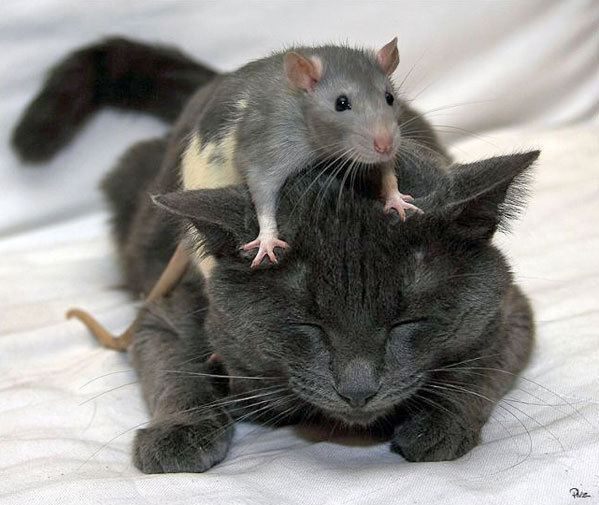
\includegraphics[width=0.35\textwidth]{figs/fast2.jpg}
%   \end{center}
%  \end{block}
% 
% \end{frame}


\begin{frame}[fragile]
\frametitle{Basic Usage: Data Management}
\begin{block}{Granularity of Operations}
 \begin{itemize}
  \item Transfer is done for each element separately
  \item High overhead, similar to scalar operations
 \end{itemize}
\end{block}

\begin{block}{How to avoid the pitfall}
 \begin{itemize}
  \item Use temporary vector
  \item Use copy functions
 \end{itemize}
   \begin{lstlisting}
viennacl::vector<double> v(10000);
std::vector<double> cpu_v( v.size() );

for (size_t i=0; i<cpu_v.size(); ++i)
  cpu_v(i) = i; 

viennacl::copy(cpu_v, v);
   \end{lstlisting}
\end{block}
\end{frame}



\begin{frame}[fragile]
\frametitle{Basic Usage: Data Management}

\begin{block}{How to access/transfer ViennaCL vectors/matrices elements?}
  \begin{itemize}
   \item Direct element access $\Rightarrow$ Bad idea!
   \item Iterator $\Rightarrow$ Bad idea!
   \item Copy functions $\Rightarrow$ \textbf{Good idea!}
  \end{itemize}
  
  \begin{lstlisting}
std::vector<ScalarType> cpu_vec(10);
viennacl::vector<ScalarType> vcl_vec(10);

for (int i = 0; i < 10; ++i)
    cpu_vec[i] = i;
    
viennacl::copy( cpu_vec, vcl_vec );

viennacl::copy( vcl_vec, cpu_vec );
  \end{lstlisting}
\end{block}

\end{frame}



\begin{frame}[fragile]
\frametitle{Basic Usage: Data Management}

\begin{block}{Fast copy}
  \begin{itemize}
   \item copy does not require linear arrays $\Rightarrow$ temporary required
   \item 
  \end{itemize}
  
  \begin{lstlisting}
std::list<ScalarType> cpu_vec(10);
viennacl::vector<ScalarType> vcl_vec(10);

for (int i = 0; i < 10; ++i)
    cpu_vec[i] = i;
    
viennacl::copy( cpu_vec, vcl_vec );

viennacl::copy( vcl_vec, cpu_vec );
  \end{lstlisting}
\end{block}

\end{frame}



\begin{frame}[fragile]
\frametitle{Basic Usage: Data Management}

\begin{block}{Fast copy}
  \begin{itemize}
   \item copy does not require linear arrays $\Rightarrow$ temporary required
   \item If container is linear memory $\Rightarrow$ use fast\_copy instead
  \end{itemize}
  
  \begin{lstlisting}
std::|\color{red}vector|<ScalarType> cpu_vec(10);
viennacl::vector<ScalarType> vcl_vec(10);

for (int i = 0; i < 10; ++i)
    cpu_vec[i] = i;
    
|\color{red}viennacl::fast\_copy( cpu\_vec, vcl\_vec );|

|\color{red}viennacl::fast\_copy( vcl\_vec, cpu\_vec );|
  \end{lstlisting}
\end{block}

\end{frame}




\begin{frame}
\frametitle{Basic Usage: Algebra}

\begin{block}{Algebra operations}
  \begin{itemize}
   \item Trivial operations done by \textbf{operator overloading}
   \item Scalar multiplication support for vector and matrices
   \item Inner product and norm support for vectors
   \item Matrix transpose using function \textbf{trans}
   \item Matrix-vector and matrix-matrix multiplication using function \textbf{prod}
  \end{itemize}
\end{block}

\end{frame}



\begin{frame}[fragile]
\frametitle{Basic Usage: Algebra}

\begin{block}{Scalar operations}
  \begin{lstlisting}
NumericType s1, s2;
viennacl::scalar<NumericType> vcl_s1, vcl_s2, vcl_s3;

vcl_s1  = 5;
vcl_s2  = vcl_s1 * 3;
vcl_s3 -= vcl_s1 + (vcl_s2 / 4);

s1      = vcl_s3;
s2      = vcl_s1 - vcl_s2 * 2;
  \end{lstlisting}
\end{block}

\end{frame}



\begin{frame}[fragile]
\frametitle{Basic Usage: Algebra}

\begin{block}{Vector operations}
  \begin{lstlisting}
viennacl::scalar<NumericType> vcl_s1, vcl_s2;
viennacl::vector<NumericType> v1(10), v2(10), v3(10);

v2  = vcl_s1 * v1 + v2
v3 += vcl_s1 * v2;

v3  = 0.5 * v2 - v3;
  \end{lstlisting}
\end{block}

\end{frame}



\begin{frame}[fragile]
\frametitle{Basic Usage: Algebra}

\begin{block}{Vector operations}
  \begin{lstlisting}
NumericType s1, s2;
viennacl::scalar<NumericType> vcl_s1, vcl_s2;
viennacl::vector<NumericType> v10), v2(10), v3(10);

vcl_s1 = viennacl::linalg::inner_prod(v1, v2);
s1     = viennacl::linalg::inner_prod(v1, v2);
 
s1     = viennacl::linalg::norm_1(v1);
vcl_s2 = viennacl::linalg::norm_2(v2);
s2     = viennacl::linalg::norm_inf(v3);
  \end{lstlisting}
\end{block}

\end{frame}



\begin{frame}[fragile]
\frametitle{Basic Usage: Algebra}

\begin{block}{Matrix operations}
  \begin{lstlisting}
viennacl::scalar<NumericType> vcl_s1, vcl_s2;
viennacl::matrix<NumericType> M1(10, 10),
    M2(10, 10), M3(10,10);

M2  = vcl_s1 * M1 + M2
M3 += vcl_s2 * M2;

M3  = 0.5 * M2 -  M3;

M3  = viennacl::trans(M2); // Transposed matrix

// Matrix-matrix product
M1  = viennacl::linalg::prod( M2, M3 );
M1  = viennacl::linalg::prod( M2, viennacl::trans(M3) );
  \end{lstlisting}
\end{block}

\end{frame}


\begin{frame}[fragile]
\frametitle{Basic Usage: Algebra}

\begin{block}{GEMM: ViennaCL vs. CUBLAS}
  \begin{lstlisting}
// ViennaCL
M1 = vcl_s1 * prod( M2, trans(M3) ) + vcl_s2 * M3;

// CUBLAS
cublasStatus_t cublasDgemm(handle,
    transa, transb,
    m, n, k,
    alpha,
    A, lda,
    B, ldb,
    beta,
    C, ldc);
  \end{lstlisting}
\end{block}

\end{frame}




\begin{frame}[fragile]
\frametitle{Basic Usage: Algebra}

\begin{block}{Matrix-vector operations}
  \begin{lstlisting}
viennacl::vector<NumericType> v1(10), v210), v3(20);
viennacl::matrix<NumericType> M1(10, 10), M2(20, 10);

v1 = viennacl::linalg::prod( M1, v2 );
v1 = viennacl::linalg::prod( viennagrid::trans(M1), v2 );
v3 = viennacl::linalg::prod( M2, v2 );
v1 = viennacl::linalg::prod( M1, v3 );
    // ERROR! dimension missmatch
  \end{lstlisting}
\end{block}

\end{frame}



\begin{frame}
\frametitle{Basic Usage: Solver}

\begin{block}{Solving a system of linear equations}
  \begin{itemize}
   \item $Ax=b$
   \item A and b given, x is unknown
   \item Common problem in mathematics
  \end{itemize}
\end{block}

\begin{block}{Types of solver}
  \begin{itemize}
   \item Direct solver
   \item Iterative solver
  \end{itemize}
\end{block}

\end{frame}



\begin{frame}
\frametitle{Basic Usage: Solver}

\begin{block}{Direct solver}
  \begin{itemize}
   \item Solving the system directly
   \item e.g. Gaussian elimination with pivoting
  \end{itemize}
\end{block}

\begin{block}{Iterative solver}
  \begin{itemize}
   \item Solving using an iterative process
   \item Convergence relies on matrix properties
   \item Recommended for large and sparse systems
   \item No write operation needed on matrix\\(most only use matrix-vector multiplication)
  \end{itemize}
\end{block}

\end{frame}



\begin{frame}[fragile]
\frametitle{Basic Usage: Solver}

\begin{block}{Direct solver}
  \begin{itemize}
   \item LU factorization
   \item No pivoting (work in progress)
  \end{itemize}
  
  \begin{lstlisting}
using namespace viennacl::linalg;

viennacl::matrix<float> vcl_matrix;
viennacl::vector<float> vcl_rhs, vcl_result;
/* Set up matrix and vectors here */

//solution of an upper triangular system:
vcl_result = solve(vcl_matrix, vcl_rhs, upper_tag());
//solution of a lower triangular system:
vcl_result = solve(vcl_matrix, vcl_rhs, lower_tag());

//solution of a full system right into the vector vcl_rhs:
lu_factorize(vcl_matrix);
lu_substitute(vcl_matrix, vcl_rhs);
  \end{lstlisting}
\end{block}

\end{frame}


\begin{frame}
\frametitle{Basic Usage: Solver}

\begin{block}{Iterative solver}
  \begin{itemize}
   \item Conjugate Gradient (CG)
   \item Stabilized Bi-CG (BiCGStab)
   \item Generalized Minimum Residual (GMRES)
  \end{itemize}
\end{block}

\begin{table}[tb]
\begin{center}
\scriptsize
\renewcommand{\arraystretch}{1.2}
\begin{tabular}{p{2.5cm}|p{1.5cm}|p{5cm}}
Method & Matrix class & ViennaCL\\
\hline
\hline
Conjugate Gradient (CG) & symmetric positive definite & \texttt{y = solve(A, x, cg\_tag());} \\
\hline
Stabilized Bi-CG (BiCGStab) & non-symmetric & \texttt{y = solve(A, x, bicgstab\_tag());} \\
\hline
Generalized Minimum Residual (GMRES) & general & \texttt{y = solve(A, x, gmres\_tag());} \\
\hline
\hline
\end{tabular}
\end{center}
\end{table}

\end{frame}



\begin{frame}[fragile]
\frametitle{Basic Usage: Solver}

\begin{block}{Iterative solver}
  \begin{itemize}
   \item Solver configuration via tag
  \end{itemize}
  
  \begin{lstlisting}
using namespace viennacl::linalg;

// conjugate gradient solver with tolerance 1e10
// and at most 100 iterations:
viennacl::linalg::cg_tag custom_cg(1e-10, 100);

vcl_result = solve(vcl_matrix, vcl_rhs, custom_cg);

//print number of iterations taken and estimated error:
cout << "No. of iters: " << custom_cg.iters() << endl;
cout << "Est. error: " << custom_cg.error() << endl;
  \end{lstlisting}
\end{block}

\end{frame}



\begin{frame}{Summary}
\begin{block}{What have we learned?}
  \begin{itemize}
   \item ViennaCL provides interface compatibility with Boost.uBLAS
   \item Basic types of ViennaCL
   \item How OpenCL kernels are used
   \item How to transfer data to and from ViennaCL
   \item How to work with ViennaCL types
   \item Simple algebraic operations
   \item Solver for systems of linear equations
  \end{itemize}
\end{block}
\end{frame}



% \begin{frame}{Summary}
% \TODO{Achievment unlocked: ViennaCL apprentice}
% \end{frame}
% 
% 
% \begin{frame}{Summary}
% \TODO{Einleitung in die Pause}
% \end{frame}